\documentclass[10pt,a4paper]{report}
\usepackage{graphicx}
\author{William Seymour}
\title{Dissertation Progress Review}
\date{\today \\ (Word count: 1000)}

\begin{document}
\maketitle

\section*{Introduction}
The project aims to explore how gamification and analytics can be used in the design of educational software. Gamification is a fairly young field of study, the term having only really gained popularity in late 2010 as shown in figure \ref{usage} (Google 2014). Its recent discovery has meant that far less has been done to incorporate developments and discoveries on gamification into the current education system. 

In addition to the study of gamification, the project also seeks to provide an example of how analytics can be used to support lecturers and allow them to better use their time when teaching in a higher education context. This will be achieved by suggesting topics and delivery methods for guided one to one or seminar style tuition in an attempt to reinforce the progress made by students online. It will also be possible to match students who share learning styles and strength/weakness pairings in specific subject areas.

Construction of a web platform capable of the aforementioned functionality is a daunting undertaking, and the research required for it to be effective in it's aims will be substantial. Taking on a project in an exciting and relatively new field is proving to be both stimulating and rewarding.

\begin{figure}
	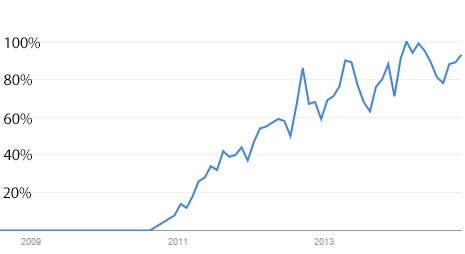
\includegraphics{../img/usage-graph.png}
	\caption{Usage of the term `gamification' by month as a proportion of the total number of google searches for gamification, from 2009 to the present day (Google 2014)}
	\label{usage}
\end{figure}

\section*{Background Research}
Before the start of term I took a MOOC entitled gamification design (Iversity, 2014), which ran over several months and included a vast array of references and resources. In addition to this, a number of other sources of information have been identified. Of particular note are those concerned with gamification in the context of higher education (Nicholson, 2013) (Niman, 2014) given that it would appear that comparatively less work has been done in this sector of the education system. Most of the work I have done so far focusses on gamification in a broader sense in order to gain a sound understanding of the topic as whole, before diving into a more in depth study of the facets specific to the project over the coming months.

It is worth studying the use of gamification in other fields, such as marketing, in order to gain additional insight into why it can be so effective, and to identify techniques which could be brought across into gamification in education. Game based marketing typically employs gamification techniques such as social networking elements and leaderboards, similar to those proposed for the project. They often find that instead of incremental gains, customer attraction and retention increases exponentially (Zichermann and Linder, 2010). 

It is also important not to forget research carried out on the `flipped classroom' model which the project follows. This is where students consume lecture material in their own time outside of school or university, instead using time spent in the classroom to ask questions and complete assessments usually done at home. Such systems often incorporate online testing and analytics like those in the project. The techniques being used to generate `significant increases in student learning and achievement' (Fulton, 2012) are being adapted for use on the aforementioned web platform, with the aim of allowing lecturers to use their time with students more effectively.

While not all of the research for the project has bee completed, taking a look at the development timeline revealed that it was more appropriate to include research for the four personality types within the timeframe allotted for their development. In this way the research can better inform the programming. However, it would be foolish to just delay this research completely. A preliminary list of sources relevant to catering for each personality type has been compiled containing documents which will form the bulk of this research. By preprocessing them in this way it is hoped that later analysis can be completed swiftly.

\section*{Technical Content}
Over the past eight weeks, work has been progressing largely according to the time line set forth in the specification. The core of the platform has been completed, including the following high level features. Figure \ref{db} contains an overview of the database which serves the project. It uses MySQL, and is currently hosted by the University's Computing Society. An overview of the classes used in the software is given in figure \ref{classes}. Database development uses phpmyadmin as installed on the Computing Society's server, which was chosen over the mysql command line interface (CLI) because it was easier to use without any prior experience, and the extra features that the CLI offers are either not required or can be exposed via running SQL commands through phpmyadmin. PHP development is done using JetBrains PHP Storm, a powerful development environment used extensively in industry. Having already had some experience using PHP Storm, it was the logical choice given how its features allow for quicker and less error prone development.

\subsection*{User Accounts}
In addition to an ID number and a username, those using the system also have persistent statistics stored and associated with their profile. This currently comprises information on their Bartle personality type, as derived from answers given to questions from course content. These values are used to generate a mask containing the users dominant personality types. Profile data is updated at the end of each module based on the answers given. A time weighted average is taken of the new scores and existing data according to a time decay constant defined in the user class. This value determines how quickly data decays in importance, or inversely, how much more relevant new data is than old data.

\subsection*{Content Creation}
There is currently basic functionality allowing the creation and deletion of content and structural database elements. The logic for this page is mainly concerned with selecting and inserting database elements correctly. If there is enough time towards the end of the project, these could be improved, but they are currently sufficient to demonstrate the other features of the software.

\subsection*{Content Delivery}
This page presents users with questions from the module they selected. Once a question has been answered, the response chosen is logged in the database, and the user is presented with the next question in the module for which they have not given an answer, or, if that was the only remaining unanswered question, the module review page. This page shows the users persistent statistics, as well as their performance on the last module they took.

\begin{figure}
	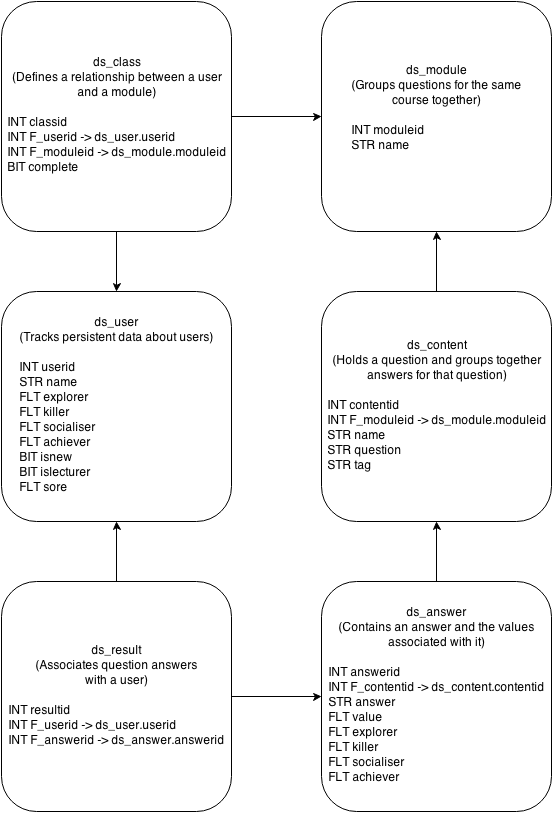
\includegraphics[width=\textwidth]{../img/database.png}
	\caption{Diagram of the current project database. Arrows denote foreign key relationships. Foreign key fields are prefixed with `F\_' and have the field they reference appended after the `-$\rangle$'.}
	\label{db}
\end{figure}

\begin{figure}
	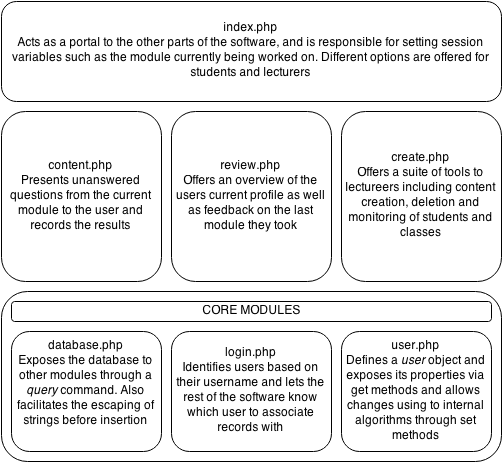
\includegraphics[width=\textwidth]{../img/classes.png}
	\caption{An overview of the classes used in the software.}
	\label{classes}
\end{figure}

\section*{Progress and Next Steps}
I realised fairly early into the term that the timetable I had submitted as part of the specification was a bit more demanding than was necessary. While it achieved its objective in that it encouraged me to work hard from the start of the project, I am currently a week behind schedule after not having enough time available to complete all the work I had hoped to. In terms of the core of the application - the components required to facilitate the gamification features - development has finished, and these features are ready to use. This will allow me to begin researching and developing the areas that are linked to each Bartle personality type. A brief explanation of these personality types is given in appendix I. In addition to development, I have also been researching the wider usage and implementation of gamification. A selection of these resources are referenced in the background research section.

After the four Bartle areas have been covered, the product will be thoroughly tested for bugs, and user feedback sought from a small focus group. Any major bugs will be fixed during this time, and any minor ones logged to be worked on should there be spare time towards the end of the project. In the focus group, a small number of people from the target demographic (undergraduate students) will be given a number of modules and asked to complete them. This data will be analysed in terms of assessing how accurately the software tracks a students user type, and how effective the tools targeted at each user were. Finally, the presentation will be delivered and the report compiled. 

\section*{Appraisal}
There was an error in the original timetable submitted in that the time set aside for writing this report was scheduled for after the due date. This, in addition to the scheduling issue mentioned above, has been rectified in a revised timetable contained in appendix II. Having a more aspirational timeline has  On reflection, I am glad that I took the time to fully assess the data that would need to be stored in the database, as once the database structure is determined it is very costly to change. As such, being able to leave it alone has saved me valuable time. The scope of the project is large, and in order to ensure its completion I have had to distil the core elements down to their simplest form in order to develop and integrate them in the allotted time. To this end, the project as it stands appears quite bare bones, but I feel that this is acceptable given that the project is more of a gamification/split classroom prototype than an exercise in rigorous software development.

\section*{Ethics}
As described in appendix I, ethical consent will have to be obtained for the user feedback testing planned for week five of term two. This approval still needs to be sought. However, as the activities proposed are eligible for devolved consent this will not take long, and will be completed by the beginning of term two.

\section*{Project Management}
In terms of project management, I have been following a variant of the incremental build model, as identified in appendix I. This has been working well, and has allowed me to timetable software development more accurately than if a more popular agile methodology had been used. The use of GitHub as a source and document control tool has been extremely useful, and it's use as a backup location has already proved invaluable once. 

TODO: Add more to this section.

\section*{Conclusion}

\section*{Appendices}

\subsection*{Appendix I - Project Specification}
\subsubsection*{Project Title}
Exploring the use of Gamification and Analytics in the Design of Educational Software.
\subsubsection*{Justification}
While the uses of gamification and teaching analytics are often explored at the levels of primary and secondary education, far less has been done to study its effects in the context of undergraduate study. Researching and determining the most effective ways to use gamification in this project will be challenging task, as gamification is still in it's infancy, the concept having only really gained popularity around 2010. In addition to this, the web application that will developed for the project will be complex. It has to manage large amounts of analytics data as well as course content, serving the needs of both students and lecturers.
\subsubsection*{Objectives}
Broadly, the goal of the project is to explore the use of gamification and advanced analytics in the development of educational software. This will be achieved through the development of an online platform allowing undergraduate students to test and enhance their understanding of course content through hybrid lectures/slides. Questions will be woven in to content delivery to provide students with rich, instant feedback on their understanding of a concept as well as additional material for extra practise. In addition, the software will categorise users into the four Bartle Test personality types (Achiever, Socialiser, Explorer and Killer) or which a brief description is given below. Users will be shown gamification elements appropriate to the users type.

The other way in which the software will aim to aid learning is in the tools presented to lecturers. Lecturers will be offered a broad overview of their modules, showing how different sections of content are being received by students. They will also be presented with detailed information on individual students, showing areas they are strong/struggling with. One example of the way in which this information can be used is to suggest content to be used as seminar content. Identifying problem areas in this way also allows for more effective use of teaching time and a better learning experience for students. Lecturers can put students who share a Bartle type together for seminars so that they can target their teaching style for maximum effectiveness.

This data can also be used to help students directly. One possible way to do this is to encourage students who are particularly strong in an area to help others who are struggling. Likewise, students who are finding a particular piece of content challenging could be prompted to seek help from colleagues who have done well at that task. By designing content assessment to be more specific than the traditional right/wrong it might be possible to give more targeted feedback and suggestions for improvement that traditional tests or assignments allow.

What follows is a brief description of the high level functionality each software component will provide. These are the components used in the development timeline below.

\subsubsection*{Core App}
The core of the application provides services such as database connectivity, objects to encapsulate users and content as well as login and authentication. It must be completed first because every subsequent task builds upon the functionality it provides.
\subsubsection*{Content Delivery}
This part of the software is responsible for reading content from the database and displaying it to the user. It also takes input from the user if the content is interactive.
\subsubsection*{Analytics}
A large part of the project revolves around capturing data about users and how they interact with the software. The analytics module is tasked with collecting and storing this data, and making inferences which can be used to offer a more engaging experience to the user (i.e. to decide which gamification elements are used).
\subsubsection*{Explorer Features}
The explorer user type is most engaged by discovering new content. This user type can be targeted with extension material to consume at the users own pace, and should not require much additional functionality, just content.
\subsubsection*{Socialiser Features}
Users who associate more with the socialiser personality type tend to seek out social experiences over anything else. To this end, the features targeted at socialisers include the ability to interact with other users who are consuming the same content, be it to give or seek help or even just discuss the task at hand.
\subsubsection*{Achiever Features}
Achievers tend to prioritise completion and progress awards when they interact with systems. The features offered to them will help them track how much of the content they have completed and offer achievements based on challenging goals.
\subsubsection*{Killer Features}
While many of the tendencies displayed by killers are not productive in an education environment, the competitiveness and desire for control they show can still be leveraged to provide an engaging experience. Features like scoreboards appeal to killers, and it may be possible to encourage them to assist other users as it puts them in a position of control.

\subsubsection*{Methodology}
The software will be web based, written in PHP, HTML, CSS and javascript, using appropriate frameworks and libraries. Github will be used for version control for both software and documents, and the repository will be synchronised with my personal webspace on the computing society's web server to allow for easy testing. User information and module content will be stored in a mySQL database, also hosted on the computing society's server.

The software development methodology used will be an adapted version of the incremental build model. Each section of the software will be developed, tested and integrated in sequence.  As the analytics part of the software (tasked with storing and updating user data, as well as making inferences based on this data) is a dependency bottleneck, the agile practise of developing a basic version first before adding features would not work. The lack of external stakeholders removes the need for frequent releases and feedback and makes the proposed methodology effective for the task at hand.

The effectiveness of the product will be determined primarily by feedback from students and staff. The exact nature of the interactions with these parties will be determined early in term two, but will definitely feature one on one sessions and interviews. The feedback provided by these sessions will form the basis for discussion on the success of the project.

\subsubsection*{Timeline}
\begin{tabular}{|c|c|}
\hline Term/Week & Tasks \\ 
\hline 1/1 & Specification \\ 
\hline 1/2 & Specification \\ 
\hline 1/3 & Core App, Environment \\ 
\hline 1/4 & Core App, Content Delivery \\ 
\hline 1/5 & Analytics \\ 
\hline 1/6 & Analytics \\ 
\hline 1/7 & Socialiser features \\ 
\hline 1/8 & Achiever features \\ 
\hline 1/9 & Killer features \\ 
\hline 1/10 & Progress Report \\ 
\hline Christmas Holiday & Buffer zone (catchup) \\
\hline 2/1 & Explorer Features \\ 
\hline 2/2 & Full product testing \\ 
\hline 2/3 & User feedback sessions \\ 
\hline 2/4 & User feedback sessions and feedback analysis \\ 
\hline 2/5 & Report \\ 
\hline 2/6 & Report \\ 
\hline 2/7 & Report \\ 
\hline 2/8 & Pesentation \\ 
\hline 2/9 & Presentation \\ 
\hline 2/10 & Presentation \\
\hline Easter Holiday & Report \\
\hline 
\end{tabular}
\subsubsection*{Dependencies for software related tasks}
\begin{tabular}{|c|c|}
\hline Task & Dependencies \\ 
\hline Core App & Specification \\ 
\hline Content Delivery & Core App \\ 
\hline Analytics & Content Delivery, Core App \\ 
\hline Explorer features & Core App, Analytics \\ 
\hline Socialiser features & Core App, Analytics \\ 
\hline Achiever features & Core App, Analytics \\ 
\hline Killer features & Core App, Analytics \\
\hline Full product testing & All of the above \\
\hline 
\end{tabular} 
\subsubsection*{Resources}
As mentioned above, the master copy of project documents and source code will be on Github. In addition, a clone of the repository will be copied after every commit to my Computing Society webspace for testing, and working copies will exist on my desktop and laptop. In terms of reliability, two of the above services could fail with no loss of data for the project. If an alternative web server is required for testing, it is possible to host the project on Joshua in the department if required. The schema and data used to create and populate the database will be added to the repository to aid recovery in the event of the database server failing. This can be uploaded to Joshua in the event of the Computing Society server failing.

When it comes to academic resources, copies of any potential papers or studies will be stored on my personal computer to provide a backup source should access to an online version be lost.
\subsubsection*{Legal, social, ethical and professional considerations}
As student and staff feedback will be required, approval will have to be sought from BSREC. As this project fulfils the conditions for delegated approval, any such activities will only have to be signed off by the project supervisor instead of being formally submitted to the committee.

\subsection*{Appendix II - Revised Timetable}
\begin{tabular}{|c|c|c|}
	\hline Term/Week & Tasks & Changed from v1 \\ 
	\hline 1/1 & Specification & No \\ 
	\hline 1/2 & Specification & No \\ 
	\hline 1/3 & Core App, Environment & No \\ 
	\hline 1/4 & Core App, Content Delivery & No \\
	\hline 1/5 & Content Delivery & Yes \\
	\hline 1/6 & Analytics & No \\ 
	\hline 1/7 & Analytics & Yes \\    
	\hline 1/8 & Progress Report & Yes \\
	\hline 1/9 & Socialiser features & Yes \\
	\hline 1/10 & Socialiser/Achiever features & Yes \\
	\hline Christmas Holiday & Buffer zone (catchup) & No \\
	\hline 2/1 & Achiever Features & Yes \\ 
	\hline 2/2 & Killer Features & Yes \\ 
	\hline 2/3 & Killer/Explorer features & Yes \\ 
	\hline 2/4 & Explorer Features & Yes \\ 
	\hline 2/5 & Product testing and feedback sessions & Yes \\ 
	\hline 2/6 & Feedback analysis & Yes \\ 
	\hline 2/7 & Report and presentation writing & Yes \\ 
	\hline 2/8 & Report and presentation writing & Yes \\ 
	\hline 2/9 & Report and presentation & Yes \\ 
	\hline 2/10 & Report and presentation & Yes \\
	\hline Easter Holiday & Report & No \\
	\hline 
\end{tabular}

\section*{Bibliography}
Google, 2014. \textit{Google Trends- Web Search interest: gamification - Worldwide, 2009 - 2014}. [image online] Available at: 

\noindent $\langle$http://www.google.com/trends/explore\#q=gamification\&date=1\%2F2009\%2072m\&cmpt=q$\rangle$ [Accessed 09/11/2014].
\newline

\noindent Iversity, 2014. \textit{Gamification Design Online Course}. [online] Available at: 

\noindent $\langle$https://iversity.org/en/courses/gamification-design-online-course$\rangle$ [Accessed 18/03/2014].
\newline

\noindent Nicholson, S., 2013. \textit{Exploring Gamification Techniques for Classroom Management}. [online] Available at: $\langle$http://scottnicholson.com/pubs/gamificationtechniquesclassroom.pdf$\rangle$ [Accessed 21/10/2014].
\newline

\noindent Niman N., 2014. \textit{The Gamification of Higher Education}. [online] Available at: $\langle$http://0-www.palgraveconnect.com.pugwash.lib.warwick.ac.uk/pc/doifinder/10.1057/9781137331465$\rangle$ [Accessed: 13 November 2014].
\newline

\noindent Zichermann, G. and Linder, J., 2010. \textit{Game-Based Marketing}. New Jersey: Wiley.
\newline

\noindent Fulton, K., 2012. \textit{Upside Down and Inside Out: Flip Your Classroom to Improve Student Learning}. [online] Available at $\langle$http://files.eric.ed.gov/fulltext/EJ982840.pdf$\rangle$ [Accessed: 13 November 2014].
\end{document}